\section{Silicon Synapses}

So far, we have seen several circuits that demonstrate fairly complex functionality by using only a small number of circuit elements. But what does this all have to do with Neuromorphic Engineering? Didn't we want to emulate the behaviour of neural systems? It turns out that by combining the previously introduced circuits we are actually able to create circuits that have very similar properties to real cortical synapses and neurons. In this chapter, we look into VLSI synapses. Make sure that you are familiar with chapter \ref{sec:neurons_synapses} and \ref{sec:perceptron} where we briefly introduced neurons and synapses as well as the Perceptron, a very simple artificial neuron model. In the Perceptron model, the synapse implements the multiplication between the neuron's input signal $X_i$ and its corresponding weight $W_i$. Silicon synapses in "classical" neural networks similarly only act as multipliers. However, we want to emulate neural systems and are therefore interested in a more biologically plausible synaptic behaviour. Biological systems communicate with spikes, i.e. short activation "pulses". So how can we generate a similar weighted pulse with our silicon synapse?

\subsection{VLSI Synapses in Pulse-based Neural Networks}

\begin{figure}
    \centering
    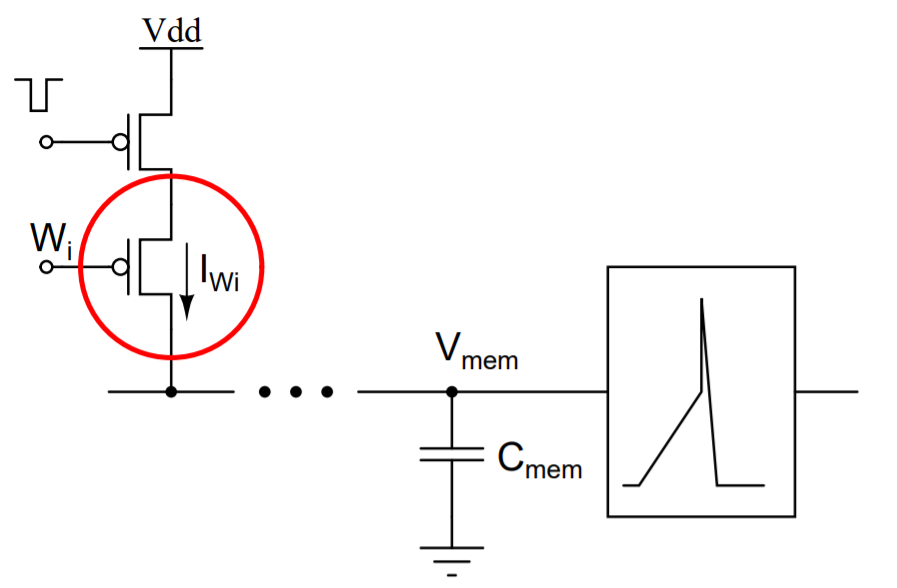
\includegraphics[width=.6\linewidth]{Figures/synapse_pulse_based_nn.PNG}
    \caption{Simple circuit of a VLSI synapse in a pulse-based neural network.}
    \label{fig:synapse_pulse_based}
\end{figure}

Figure \ref{fig:synapse_pulse_based} demonstrates the simplest circuit to generate an output pulse. It consists of two pFET transistors and one capacitor. The pFET MOSFET on the top receives an input in the form of a gate voltage change. By decreasing the gate voltage, a current is generated. The strength of the current is shaped by the lower pFET whose gate voltage $W_i$ we can adjust. The generated current $I_{wi}$ finally charges the circuit's capacitor and the charging and the discharging of the capacitor creates our desired voltage "spike" as shown on the right. Based on the capacitor equation $C\frac{dV}{dt} = I$, we can describe the voltage change as follows:

\begin{equation}
    \Delta V_i = \frac{I_{wi}}{C_{mem}} \Delta t
\end{equation}

The above equation demonstrates that the strength of the output spike can be changed by either changing the bias voltage $W_i$ which shapes the current $I_{wi}$ or by changing the duration $\Delta t$ of the input. The demonstrated circuit allows us to implement an excitatory synapse. By replacing the pFETs with two nFETs (connected to ground instead of $V_{dd}$), the generated current $I_{wi}$ flows into the opposite direction. The capacitor is consequently discharged first and we get an inhibitory synapse. As we are using a current source - our $I_{wi}$ - to (dis)charge the capacitor, the voltage changes linearly. This is however not biologically plausible. In biological systems, a synapse acts as a linear integrator. If you recall chapter \ref{sec:resistor_capcitor_circuits}, an integrator is equivalent to a low-pass filter. Its impulse response is a decaying exponential. Remember that in subthreshold, there is an exponential relationship between the voltage and the current, e.g. as shown in the equation of a saturated pFET in subthreshold:

\begin{equation}
    I(t) = I_0 e^{\frac{\kappa}{U_T}(V_{dd}-V_g(t))}
\end{equation}

If we linearly change the gate voltage, we get an exponential change of current. So let's use this intrinsic property of subthreshold MOSFETs to build a biologically plausible synapse.

\subfile{Exponentially_Decaying_Integrator.tex}
\subfile{Log_Domain_Pulse_Integrator.tex}
\subfile{Diff_Pair_Integrator.tex}
\subfile{Lab-08Synapses.tex}